\documentclass{article}
\usepackage[T1]{fontenc}
\usepackage{lmodern}
\usepackage{graphicx}
\usepackage{amsmath,amssymb}
\usepackage[a4paper,margin=2cm]{geometry}
\usepackage[absolute,overlay]{textpos}
\setlength{\TPHorizModule}{1mm}
\setlength{\TPVertModule}{1mm}
\usepackage[indonesian]{babel}
\usepackage{hyperref}
\setlength{\emergencystretch}{2em}
% unit: Halaman 17

\begin{document}

% === Halaman 17 (python/native) ===

17

Giovanni Battista Porta

(1535-1615 )

Giovanni Battista Porta menggambarkan cara 

menyembunyikan pesan di dalam telur rebus.

Caranya, pesan ditulis pada kulit telur yang dibuat 

dari tinta khusus yang dibuat dengan satu ons 

tawas dan setengah liter cuka. 

Prinsipnya penyembunyiannya adalah tinta 

tersebut akan menembus kulit telur yang berpori, 

tanpa meninggalkan jejak yang terlihat.

Tulisan dari tinta akan membekas pada permukaan isi telur yang telah mengeras 

(karena sudah direbus sebelumnya). Pesan dibaca dengan membuang kulit telur

% deskripsi: gambar native xref 116
\noindent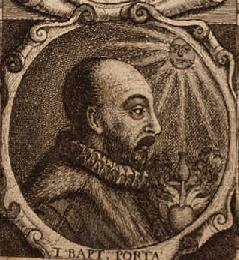
\includegraphics[width=0.85\textwidth]{../../images/python/page_017_img_01.jpeg}

\end{document}
